
% RUN:
% pdflatex -output-directory=/home/salvadortorpes/Aprendizagem/Homework1/trash /home/salvadortorpes/Aprendizagem/Homework1/G22.tex

% ir a settings.json e adicionar:
% // According to the wiki, the string latex-workshop.latex.autoBuild.run has three possible values: never, onSave and onFileChange(default).
% "latex-workshop.latex.autoBuild.run": "never",

\documentclass{article}

\author{Pedro Curvo (ist1102716) $|$ Salvador Torpes (ist1102474)}

\usepackage[utf8]{inputenc}
\usepackage[portuguese]{babel}
% \usepackage[letterpaper,top=10mm,bottom=15mm,left=15mm,right=15mm,marginparwidth=1.75cm]{geometry}
% \usepackage[letterpaper,top=10mm,bottom=15mm,left=15mm,right=15mm,marginparwidth=1.75cm]{geometry}
\usepackage[letterpaper,margin=1in,marginparwidth=1.75cm]{geometry}
\usepackage{multicol}
\usepackage{biblatex}
\addbibresource{Bibliografia.bib}
\usepackage{graphicx}
% \graphicspath{{../Homework1/images/}}
\usepackage{subcaption}
\usepackage{tabularx}
\usepackage{booktabs}
\usepackage{array}
\usepackage{makecell}
\usepackage{multirow}
\usepackage{amsmath}
\usepackage{makecell}
\usepackage{url}
\usepackage{csquotes}
\usepackage{caption}
\usepackage{enumitem}
\usepackage{textcomp}
\usepackage{pdflscape}
\usepackage{makeidx}
\usepackage{amsmath}
% \usepackage{tocbibind}
\providecommand{\tightlist}{\relax}
\usepackage{tocloft}
\renewcommand{\cftsecindent}{0em}
\renewcommand{\cftsubsecindent}{1em}
\renewcommand{\cftsecfont}{\bfseries}
\renewcommand{\cftsubsecfont}{\itshape}
\setlength{\cftsubsecnumwidth}{0em}

\usepackage[version=4]{mhchem}
\usepackage{hyperref} % Remove "pdftex" option here
\usepackage{float}
\usepackage{fancyhdr}
\usepackage{ragged2e}
\usepackage{xkeyval}
%\usepackage{minted}
%\usemintedstyle{manni}
\usepackage{listings}
\usepackage{amssymb}




\usepackage{tikz}
\usetikzlibrary{positioning}
\usetikzlibrary{positioning, arrows.meta}
\usepackage{adjustbox}
\usepackage{sidecap}



% \usepackage[table,xcdraw]{xcolor}
\usepackage[LY1]{fontenc}
\usepackage{tikz-3dplot}
% \usepackage{pgfplots}
\usetikzlibrary{calc, 3d, arrows}
\usepackage{forest}




\usetikzlibrary{shapes.geometric, arrows}


\lstset{
    language=Python,
    basicstyle=\ttfamily,
    keywordstyle=\color{blue},
    commentstyle=\color{gray},
    stringstyle=\color{orange},
    numbers=left,
    numberstyle=\tiny,
    numbersep=5pt,
    showspaces=false,
    showstringspaces=false,
    breaklines=true,
    frame=tb,
    framexleftmargin=2em,
    xleftmargin=2em,
}


%\usepackage{fontspec}

%\setmonofont{Fira Code}

\fancyhf{}
\cfoot{\thepage}
\fancyhf{} % Clear all header and footer fields
\renewcommand{\headrulewidth}{0pt} % Remove the header rule line
\cfoot{\thepage} % Set the page number in the center of the footer

\pagestyle{fancy} % Apply the fancy page style

\setlength\columnsep{20pt}

\renewcommand{\familydefault}{\sfdefault}

\newenvironment{Figure}
  {\par\medskip\noindent\minipage{\linewidth}}
  {\endminipage\par\medskip}

\makeatletter
\newenvironment{figurehere}
{\def\@captype{figure}}
{}
\makeatother

\hypersetup{
  colorlinks,
  linkcolor=blue,
  anchorcolor=black,
  citecolor=cyan,
  filecolor=cyan,
  menucolor=cyan,
  urlcolor=cyan,
  bookmarksopen=true,
  bookmarksnumbered=true
}

\makeindex


\title{\vspace{-6mm}
\includegraphics[width=15mm,scale=2]{images/IST_Logo.png}\\ \vspace{5mm}
Aprendizagem - Homework 1 \vspace{-5mm}}
\date{1º Semestre - 23/24}

\usepackage{sansmathfonts}
\usepackage[T1]{fontenc}
\usepackage[OT1]{fontenc}

\usepackage{listings}
\usepackage{xcolor}

\definecolor{codegreen}{rgb}{0,0.6,0}
\definecolor{codegray}{rgb}{0.5,0.5,0.5}
\definecolor{codepurple}{rgb}{0.58,0,0.82}
\definecolor{backcolour}{rgb}{0.95,0.95,0.92}

\lstdefinestyle{mystyle}{
  backgroundcolor=\color{backcolour},   
  commentstyle=\color{codegray},
  keywordstyle=\color{magenta},
  numberstyle=\tiny\color{codegray},
  stringstyle=\color{codegreen},
  keywordstyle=[2]{\color{orange}},
  keywords=[2]{plt.},
  basicstyle=\ttfamily\footnotesize,
  breakatwhitespace=false,         
  breaklines=true,                 
  captionpos=b,                    
  keepspaces=true,                 
  numbers=left,                    
  numbersep=5pt,                  
  showspaces=false,                
  showstringspaces=false,
  showtabs=false,                  
  tabsize=2,
  frame=single,
  framesep=2pt,
  framerule=0pt,
  xleftmargin=2pt,
  xrightmargin=2pt,
  aboveskip=1em,
  belowskip=1em,
  abovecaptionskip=0.5em,
  belowcaptionskip=0.5em,
  caption=\lstname,
  captionpos=b,
  language=Python,
  morekeywords={as},
  deletekeywords={None},
  emph={self},
  emphstyle=\color{blue},
  escapeinside={(*@}{@*)},
  literate={+}{{\textcolor{blue}{+}}}1
       {*}{{\textcolor{blue}{*}}}1
       {-}{{\textcolor{blue}{-}}}1
       {/}{{\textcolor{blue}{/}}}1
       {=}{{\textcolor{blue}{=}}}1
       {>}{{\textcolor{blue}{>}}}1
       {<}{{\textcolor{blue}{<}}}1
       {==}{{\textcolor{blue}{==}}}2
       {!=}{{\textcolor{blue}{!=}}}2
       {<=}{{\textcolor{blue}{<=}}}2
       {>=}{{\textcolor{blue}{>=}}}2,
  }
    
    \lstset{style=mystyle}
    \usepackage{fancyhdr}
    
    % Define header and footer styles
    \fancypagestyle{plain}{%
      \fancyhf{}% Clear header/footer
      \fancyhead[L]{Homework 1}% Header left
      \fancyhead[C]{2023/2024}% Header left
      \fancyhead[R]{Aprendizagem}% Header right
      \fancyfoot[C]{\thepage}% Footer center
      \renewcommand{\headrulewidth}{0.4pt}% Header rule
      \renewcommand{\footrulewidth}{0pt}% Footer rule
    }
    
    % Apply the style to all pages except the first one
    \pagestyle{plain}
    \thispagestyle{empty} % Remove header/footer from first page
    
\begin{document}
    
    \renewcommand{\arraystretch}{1.7}
    \setlength{\columnseprule}{0.4pt}
    \tdplotsetmaincoords{70}{110} % Set the viewing angle
    \newcolumntype{M}[1]{>{\centering\arraybackslash\vspace{#1}}m{0.5\linewidth}<{\vspace{#1}}}
    \newcolumntype{C}[2]{>{\centering\arraybackslash\vspace{#1}\rule{0pt}{#1}\hspace{0pt}}m{#2}}
    \ifx\undefined\w
    \newcolumntype{w}[1]{>{\centering\arraybackslash}m{#1}}
    \fi
    
    \renewcommand*\familydefault{\sfdefault} %% Only if the base font of the document is to be sans serif
    
    \maketitle
    
    \vspace{-5mm}
    
    \hrulefill
    \section*{Dataset}
    
    
    Consideramos o seguinte dataset D:
    
    \begin{table}[h!]
      \centering
      \begin{tabular}{|c|c|c|c|c|c|}
        \hline
        D     & $y_1$ & $y_2$ & $y_3$ & $y_4$ & $y_{out}$ \\ \hline
        $x_1$ & 0.24   & 1     & 1     & 0     & A         \\ \hline
        $x_2$ & 0.06   & 2     & 0     & 0     & B         \\ \hline
        $x_3$ & 0.04   & 0     & 0     & 0     & B         \\ \hline
    $x_4$ & 0.36   & 0     & 2     & 1     & C         \\ \hline
    $x_5$ & 0.32   & 0     & 0     & 2     & C         \\ \hline
    $x_6$ & 0.68   & 2     & 2     & 1     & A         \\ \hline
    $x_7$ & 0.90   & 0     & 1     & 2     & A         \\ \hline
    $x_8$ & 0.76   & 2     & 2     & 0     & A         \\ \hline
    $x_9$ & 0.46   & 1     & 1     & 1     & B         \\ \hline
    $x_{10}$ & 0.62   & 0     & 0     & 1     & B         \\ \hline
    $x_{11}$ & 0.44   & 1     & 2     & 2     & C         \\ \hline
    $x_{12}$ & 0.52   & 0     & 2     & 0     & C         \\ \hline
  \end{tabular}
  \caption{Dataset D}
  \label{tab:datasetD}
\end{table}

\newpage

\section*{Exercício 1.}

De modo a corretamente completar a árvore de decisão, é necessário calcular o Information gain (IG) da variável de output $y_{out}$ condicionada a cada uma das variáveis $y_2$, $y_3$ e $y_4$. 
Temos de repetir o processo para cada nó.

\subsection*{Escolha do 2º nó}

Como queremos completar o ramo $y_1>0.4$, vamos apenas considerar as ocorrências em que $y_1>0.4$ para calcular o IG.

\paragraph{Information Gain de $y_{out}$ condicionada a $y_2$}

\[ IG(y_{out}|y_2) = H(y_{out}) - H(y_{out}|y_2) \]

\[ H(y_{out}) = \left(- \sum_{i=1}^{3} p_{out_i} (\log_2 p_{out_i})\right) = - \left( \frac{3}{7} \log_2 \left( \frac{3}{7} \right) + \frac{2}{7} \log_2 \left( \frac{2}{7} \right) + \frac{2}{7} \log_2 \left( \frac{2}{7} \right) \right) = 1.5567 \]

\[ H(y_{out}|y_2) = \sum_{i=0}^{2} p_{y_2 = i} H(y_{out}|y_2 = i) \]

Tabela dividida em 3 sub-tabelas, cada uma com os dados que verificam $y_2 = 0$, $y_2 = 1$ e $y_2 = 2$, respetivamente:

\begin{center}
\begin{minipage}[b]{0.3\linewidth}
  \centering
  \begin{table}[H]
    \centering
    \begin{tabular}{|c|c|c|}
        \hline
        D     & $y_2$ & $y_{out}$ \\ \hline
        $x_7$ & 0     & A         \\ \hline
        $x_{10}$ & 0     & B         \\ \hline
        $x_{12}$ & 0     & C         \\ \hline
    \end{tabular}
    \caption{Dataset D com $y_2 = 0$}
    \label{tab:datasetDy2=0}
  \end{table}
\end{minipage}
\begin{minipage}[b]{0.3\linewidth}
  \centering
  \begin{table}[H]
    \centering
    \begin{tabular}{|c|c|c|}
      \hline
        D     & $y_2$ & $y_{out}$ \\ \hline
        $x_9$ & 1     & B         \\ \hline
        $x_{11}$ & 1     & C         \\ \hline
    \end{tabular}
    \caption{Dataset D com $y_2 = 1$}
    \label{tab:datasetDy2=1}
  \end{table}
\end{minipage}
\begin{minipage}[b]{0.3\linewidth}
  \centering
  \begin{table}[H]
    \centering
    \begin{tabular}{|c|c|c|}
    \hline
        D     & $y_2$ & $y_{out}$ \\ \hline
        $x_6$ & 2     & A         \\ \hline
        $x_8$ & 2     & A         \\ \hline
    \end{tabular}
    \caption{Dataset D com $y_2 = 2$}
    \label{tab:datasetDy2=2}
  \end{table}
\end{minipage}
\end{center}

\[ H(y_{out}|y_2 = 0) = - \left( \frac{1}{3} \log_2 \left( \frac{1}{3} \right) + \frac{1}{3} \log_2 \left( \frac{1}{3} \right) + \frac{1}{3} \log_2 \left( \frac{1}{3} \right) \right) = 1.58496 \]

\[ H(y_{out}|y_2 = 1) = - \left( \frac{1}{2} \log_2 \left( \frac{1}{2} \right) + \frac{1}{2} \log_2 \left( \frac{1}{2} \right) \right) = 1 \]

\[ H(y_{out}|y_2 = 2) = - \left( \log(1) \right) = 0 \]

Assim, podemos calcular a entropia de $y_{out}$ condicionada a $y_2$:

\[ H(y_{out}|y_2) = \frac{3}{7} H(y_{out}|y_2 = 0) + \frac{2}{7} H(y_{out}|y_2 = 1) + \frac{2}{7} H(y_{out}|y_2 = 2) = \]
\[ = \frac{3}{7} \times 1.58496 + \frac{2}{7} \times 1 + \frac{2}{7} \times 0 = 0.96498 \]

Por fim, podemos calcular o Information Gain:

\[ IG(y_{out}|y_2) = H(y_{out}) - H(y_{out}|y_2) = 1.5567 - 0.96498 = 0.59172 \]

\paragraph{Information Gain de $y_{out}$ condicionada a $y_3$}

\[ IG(y_{out}|y_3) = H(y_{out}) - H(y_{out}|y_3) \]

\[ H(y_{out}|y_3) = \sum_{i=0}^{2} p_{y_3 = i} H(y_{out}|y_3 = i) \]

Tabela dividida em 3 sub-tabelas, cada uma com os dados que verificam $y_3 = 0$, $y_3 = 1$ e $y_3 = 2$, respetivamente:

\begin{center}
\begin{minipage}[b]{0.3\linewidth}
  \centering
  \begin{table}[H]
    \centering
    \begin{tabular}{|c|c|c|}
      \hline
      D     & $y_3$ & $y_{out}$ \\ \hline
      $x_{10}$ & 0     & B         \\ \hline
    \end{tabular}
    \caption{Dataset D com $y_3 = 0$}
    \label{tab:datasetDy3=0}
  \end{table}
\end{minipage}
\begin{minipage}[b]{0.3\linewidth}
  \centering
  \begin{table}[H]
    \centering
    \begin{tabular}{|c|c|c|}
      \hline
      D     & $y_3$ & $y_{out}$ \\ \hline
      $x_7$ & 1     & A         \\ \hline
      $x_9$ & 1     & B         \\ \hline
    \end{tabular}
    \caption{Dataset D com $y_3 = 1$}
    \label{tab:datasetDy3=1}
  \end{table}
\end{minipage}
\begin{minipage}[b]{0.3\linewidth}
  \centering
  \begin{table}[H]
    \centering
    \begin{tabular}{|c|c|c|}
      \hline
      D     & $y_3$ & $y_{out}$ \\ \hline
      $x_6$ & 2     & A         \\ \hline
      $x_8$ & 2     & A         \\ \hline
      $x_{11}$ & 2     & C         \\ \hline
      $x_{12}$ & 2     & C         \\ \hline
    \end{tabular}
    \caption{Dataset D com $y_3 = 2$}
    \label{tab:datasetDy3=2}
  \end{table}
\end{minipage}
\end{center}


\[ H(y_{out}|y_3 = 0) = - \left( \log(1) \right) = 0 \]

\[ H(y_{out}|y_3 = 1) = - \left( \frac{1}{2} \log_2 \left( \frac{1}{2} \right) + \frac{1}{2} \log_2 \left( \frac{1}{2} \right) \right) = 1 \]

\[ H(y_{out}|y_3 = 2) = - \left( \frac{2}{4} \log_2 \left( \frac{2}{4} \right) + \frac{2}{4} \log_2 \left( \frac{2}{4} \right) \right) = 1 \]

Assim, podemos calcular a entropia de $y_{out}$ condicionada a $y_3$:

\[ H(y_{out}|y_3) = \frac{1}{7} H(y_{out}|y_3 = 0) + \frac{2}{7} H(y_{out}|y_3 = 1) + \frac{4}{7} H(y_{out}|y_3 = 2) = \]

\[ = \frac{1}{7} \times 0 + \frac{2}{7} \times 1 + \frac{4}{7} \times 1 = 0.85714 \]

Por fim, podemos calcular o Information Gain:

\[ IG(y_{out}|y_3) = H(y_{out}) - H(y_{out}|y_3) = 1.5567 - 0.85714 = 0.69956 \]

\paragraph{Information Gain de $y_{out}$ condicionada a $y_4$}

\[ IG(y_{out}|y_4) = H(y_{out}) - H(y_{out}|y_4) \]

\[ H(y_{out}|y_4) = \sum_{i=0}^{2} p_{y_4 = i} H(y_{out}|y_4 = i) \]

Tabela dividida em 3 sub-tabelas, cada uma com os dados que verificam $y_4 = 0$, $y_4 = 1$ e $y_4 = 2$, respetivamente:

\begin{center}
\begin{minipage}[b]{0.3\linewidth}
  \centering
  \begin{table}[H]
    \centering
    \begin{tabular}{|c|c|c|}
      \hline  
      D     & $y_4$ & $y_{out}$ \\ \hline
      $x_8$ & 0     & A         \\ \hline
      $x_{12}$ & 0     & C         \\ \hline
    \end{tabular}
    \caption{Dataset D com $y_4 = 0$}
    \label{tab:datasetDy4=0}
  \end{table}
\end{minipage}
\begin{minipage}[b]{0.3\linewidth}
  \centering
  \begin{table}[H]
    \centering
    \begin{tabular}{|c|c|c|}
      \hline
      D     & $y_4$ & $y_{out}$ \\ \hline
      $x_6$ & 1     & A         \\ \hline
      $x_9$ & 1     & B         \\ \hline
      $x_{10}$ & 1     & B         \\ \hline
      \end{tabular}
    \caption{Dataset D com $y_4 = 1$}
    \label{tab:datasetDy4=1}
  \end{table}
\end{minipage}
\begin{minipage}[b]{0.3\linewidth}
  \centering
  \begin{table}[H]
    \centering
    \begin{tabular}{|c|c|c|}
      \hline
      D     & $y_4$ & $y_{out}$ \\ \hline
      $x_7$ & 2     & A         \\ \hline
      $x_{11}$ & 2     & C         \\ \hline
    \end{tabular}
    \caption{Dataset D com $y_4 = 2$}
    \label{tab:datasetDy4=2}
  \end{table}
\end{minipage}
\end{center}

\[ H(y_{out}|y_4 = 0) = - \left( \frac{1}{2} \log_2 \left( \frac{1}{2} \right) + \frac{1}{2} \log_2 \left( \frac{1}{2} \right) \right) = 1 \]

\[ H(y_{out}|y_4 = 1) = - \left( \frac{2}{3} \log_2 \left( \frac{2}{3} \right) + \frac{1}{3} \log_2 \left( \frac{1}{3} \right) \right) = 0.918295 \]

\[ H(y_{out}|y_4 = 2) = - \left( \frac{1}{2} \log_2 \left( \frac{1}{2} \right) + \frac{1}{2} \log_2 \left( \frac{1}{2} \right) \right) = 1 \]

Assim, podemos calcular a entropia de $y_{out}$ condicionada a $y_4$:

\[ H(y_{out}|y_4) = \frac{2}{7} H(y_{out}|y_4 = 0) + \frac{3}{7} H(y_{out}|y_4 = 1) + \frac{2}{7} H(y_{out}|y_4 = 2) = \]

\[ = \frac{2}{7} \times 1 + \frac{3}{7} \times 0.918295 + \frac{2}{7} \times 1 = 0.96498 \]

Por fim, podemos calcular o Information Gain:

\[ IG(y_{out}|y_4) = H(y_{out}) - H(y_{out}|y_4) = 1.5567 - 0.96498 = 0.59172 \]

\paragraph{Comparação dos IG}

Podemos confirmar, pelos cálculos acima, que:

\[ IG(y_{out}|y_2) = IG(y_{out}|y_4) < IG(y_{out}|y_3) \]

Assim, a variável $y_3$ é a que tem maior IG, pelo que é a variável que escolhemos para o 2º nó da árvore de decisão no ramo $y_1>0.4$.
Este nó vai ter três ramos, um para cada valor possível de $y_3$: o caso $y_3=0$ tem apenas uma ocorrência e $y_3=1$ apenas tem duas, pelo que estes dois ramos não são expandidos numa nova variável de input.
Por outro lado, $y_3=2$ tem 4 ocorrências, pelo que é o único nó que é expandido numa nova variável de input. Falta averiguar qual a variável que vai ser usada para expandir este nó.

\subsection*{Escolha do 3º nó}

Queremos agora completar o ramo que verifica $y_1 > 0.4$ e $y_3 = 2$. Para isso, vamos calcular o IG de $y_{out}$ condicionada a $y_2$ e $y_4$ considerando apenas as ocorrências que verificam $y_1 > 0.4$ e $y_3 = 2$:

\paragraph{Information Gain de $y_{out}$ condicionada a $y_2$}

\[ IG(y_{out}|y_2) = H(y_{out}) - H(y_{out}|y_2) \]

\[ H(y_{out}) = \left(- \sum_{i=1}^{3} p_{out_i} (\log_2 p_{out_i})\right) = - \left( \frac{2}{4} \log_2 \left( \frac{2}{4} \right) + \frac{2}{4} \log_2 \left( \frac{2}{4} \right) \right) = 1 \]

\[ H(y_{out}|y_2) = \sum_{i=0}^{2} p_{y_2 = i} H(y_{out}|y_2 = i) \]

As entropias condicionadas de $y_{out}$ para cada valor de $y_2$ são:

\[ H(y_{out}|y_2 = 0) = - \left( \log_2(1) \right) = 0 \]

\[ H(y_{out}|y_2 = 1) = - \left( \log_2(1) \right) = 0 \]

\[ H(y_{out}|y_2 = 2) = - \left( \log_2(1) \right) = 0 \]

Assim, podemos calcular a entropia de $y_{out}$ condicionada a $y_2$:

\[ H(y_{out}|y_2) = \frac{1}{4} H(y_{out}|y_2 = 0) + \frac{1}{4} H(y_{out}|y_2 = 1) + \frac{2}{4} H(y_{out}|y_2 = 2) = \]

\[ = \frac{1}{4} \times 0 + \frac{1}{4} \times 0 + \frac{2}{4} \times 0 = 0 \]

Por fim, podemos calcular o Information Gain:

\[ IG(y_{out}|y_2) = H(y_{out}) - H(y_{out}|y_2) = 1 - 0 = 1 \]

\paragraph{Information Gain de $y_{out}$ condicionada a $y_4$}

\[ IG(y_{out}|y_4) = H(y_{out}) - H(y_{out}|y_4) \]

\[ H(y_{out}|y_4) = \sum_{i=0}^{2} p_{y_4 = i} H(y_{out}|y_4 = i) \]

As entropias condicionadas de $y_{out}$ para cada valor de $y_4$ são:

\[ H(y_{out}|y_4 = 0) = - \left( \frac{1}{2} \log_2 \left( \frac{1}{2} \right) + \frac{1}{2} \log_2 \left( \frac{1}{2} \right) \right) = 1 \]

\[ H(y_{out}|y_4 = 1) = - \left( \log_2(1) \right) = 0 \]

\[ H(y_{out}|y_4 = 2) = - \left( \log_2(1) \right) = 0 \]

Assim, podemos calcular a entropia de $y_{out}$ condicionada a $y_4$:

\[ H(y_{out}|y_4) = \frac{2}{4} H(y_{out}|y_4 = 0) + \frac{1}{4} H(y_{out}|y_4 = 1) + \frac{1}{4} H(y_{out}|y_4 = 2) = \]

\[ = \frac{2}{4} \times 1 + \frac{1}{4} \times 0 + \frac{1}{4} \times 0 = 0.5 \]

Por fim, podemos calcular o Information Gain:

\[ IG(y_{out}|y_4) = H(y_{out}) - H(y_{out}|y_4) = 1 - 0.5 = 0.5 \]

\paragraph{Comparação dos IG}

Podemos confirmar, pelos cálculos acima, que:

\[ IG(y_{out}|y_2) > IG(y_{out}|y_4) \]

Assim, a variável $y_2$ é a que tem maior IG, pelo que é a variável que escolhemos para o 3º nó da árvore de decisão no ramo $y_1>0.4$ e $y_3 = 2$.
Todos os ramos deste nó têm menos que 4 ocorrências, pelo que nehum deles é expandido e termina a árvore de decisão.

\subsection*{Construção da árvore de decisão}

Para completar a árvore, resta preencher os nós terminais com os valores de $y_{out}$ que são mais prováveis em cada ramo. Em caso de empate, escolhemos por ordem alfabética.
A árvore de decisão final é:

\begin{center}
  \begin{forest}
    for tree={
      edge={->},
      parent anchor=south,
      child anchor=north,
      align=center,
      base=top,
      draw,
      font=\sffamily,
      s sep=9mm, % Vertical separation between siblings
      l sep=10mm, % Horizontal separation between parent and child nodes
    }
    [$y_1$, circle
      [$y_2$, edge label={node[midway,above]{ $ \leq 0.4$}}, circle
        [C, diamond, label = {$ = 0$}]
        [A, diamond, label = {$ = 1$}]
        [B, diamond, label = {$ = 2$}]
      ]
      [$y_3$, edge label={node[midway,above]{ $ > 0.4$}}, circle
        [B, diamond, label = {$ = 0$}]
        [A, diamond, label = {$ = 1$}]
        [$y_2$, circle, label = {$ = 2$}
          [C, diamond, label = {$ = 0$}]
          [C, diamond, label = {$ = 1$}]
          [A, diamond, label = {$ = 2$}]
        ]
      ]
    ]
  % \caption{Árvore de decisão Final}
  \end{forest}
  
\end{center}

\newpage

\section*{Exercício 2.}

Com o objetivo de desenhar a matriz de confusão da árvore de decisão construída acima, começamos por calcular os valores previstos para o output, $\hat{y}_{out}$, para cada uma das ocorrências do dataset D:

\begin{table}[h!]
  \centering
  \begin{tabular}{|c|c|c|c|c|c|c|}
    \hline
        D     & $y_1$ & $y_2$ & $y_3$ & $y_4$ & $\hat{y}_{out}$ & $y_{out}$ \\ \hline
        $x_1$ & 0.24   & 1     & 1     & 0     & A         & A         \\ \hline
        $x_2$ & 0.06   & 2     & 0     & 0     & B         & B         \\ \hline
        $x_3$ & 0.04   & 0     & 0     & 0     & C         & B         \\ \hline
        $x_4$ & 0.36   & 0     & 2     & 1     & C         & C         \\ \hline
        $x_5$ & 0.32   & 0     & 0     & 2     & C         & C         \\ \hline
        $x_6$ & 0.68   & 2     & 2     & 1     & A         & A         \\ \hline
        $x_7$ & 0.90   & 0     & 1     & 2     & A         & A         \\ \hline
        $x_8$ & 0.76   & 2     & 2     & 0     & A         & A         \\ \hline
        $x_9$ & 0.46   & 1     & 1     & 1     & A         & B         \\ \hline
        $x_{10}$ & 0.62   & 0     & 0     & 1     & B         & B         \\ \hline
        $x_{11}$ & 0.44   & 1     & 2     & 2     & C         & C         \\ \hline
        $x_{12}$ & 0.52   & 0     & 2     & 0     & C         & C         \\ \hline
    \end{tabular}
  \caption{Dataset D com $\hat{y}_{out}$}
  \label{tab:datasetD_comprev}
\end{table}

Assim, desenhamos a \textbf{matriz de confusão}:



  \begin{table}[H]
    \centering
    \begin{tabular}{|c|cccc|}
      \hline
        & \multicolumn{4}{c|}{Valores reais}                                           \\ \hline
      \multirow{4}{*}{\rotatebox[origin=c]{90}{Valores Previstos}} & \multicolumn{1}{c|}{} & \multicolumn{1}{c|}{A} & \multicolumn{1}{c|}{B} & C \\ \cline{2-5} 
        & \multicolumn{1}{c|}{A} & \multicolumn{1}{c|}{4} & \multicolumn{1}{c|}{1} & 0 \\ \cline{2-5} 
        & \multicolumn{1}{c|}{B} & \multicolumn{1}{c|}{0} & \multicolumn{1}{c|}{2} & 0 \\ \cline{2-5} 
        & \multicolumn{1}{c|}{C} & \multicolumn{1}{c|}{0} & \multicolumn{1}{c|}{1} & 4 \\ \hline
    \end{tabular}
    \caption{Matriz de confusão}
    \label{tab:confusion_matrix}
  \end{table}





\newpage

\section*{Exercício 3.}

Para calcular o $F_1$-score para cada uma das classes de $y_{out}$, começamos por calcular a precisão e o recall para cada uma delas:

A precisão é dada por:
\[ P = \frac{TP}{TP + FP} \]
Onde $TP$ é o número de true positives e $FP$ é o número de false positives.
O recall é dado por:
\[ R = \frac{TP}{TP + FN} \]
Onde $FN$ é o número de false negatives.
\paragraph{}

Assim, obtemos que:
\begin{center}
  \begin{minipage}{0.3\textwidth}
    \begin{align*}
      P_A &= \frac{4}{4 + 1 + 0} = \frac{4}{5} \\
      R_A &= \frac{4}{4 + 0 + 0} = 1 \\
    \end{align*}
  \end{minipage}
  \begin{minipage}{0.3\textwidth}
    \begin{align*}
      P_B &= \frac{2}{2 + 0 + 0} = 1 \\
      R_B &= \frac{2}{2 + 1 + 1} = \frac{1}{2} \\
    \end{align*}
  \end{minipage}
  \begin{minipage}{0.3\textwidth}
    \begin{align*}
      P_C &= \frac{4}{4 + 1 + 0} = \frac{4}{5} \\
      R_C &= \frac{4}{4 + 0 + 0} = 1 \\
    \end{align*}
  \end{minipage}
\end{center}

Por fim, o $F_1$-score é dado por:

\[ F_1 = \frac{1}{0.5\cdot \frac{1}{P} + 0.5\cdot \frac{1}{R}} \]

Assim, podemos calcular o $F_1$-score para cada uma das classes:

\[ F_1(A) = \frac{1}{0.5\cdot \frac{5}{4} + 0.5\cdot 1} = \frac{1}{\frac{5}{8} + \frac{1}{2}} = \frac{1}{\frac{5}{8} + \frac{4}{8}} = \frac{1}{\frac{9}{8}} = \frac{8}{9} \]

\[ F_1(B) = \frac{1}{0.5\cdot 1 + 0.5\cdot 2} = \frac{1}{0.5 + 1} = \frac{1}{1.5} = \frac{2}{3} \]

\[ F_1(C) = \frac{1}{0.5\cdot \frac{5}{4} + 0.5\cdot 1} = \frac{1}{\frac{5}{8} + \frac{1}{2}} = \frac{1}{\frac{5}{8} + \frac{4}{8}} = \frac{1}{\frac{9}{8}} = \frac{8}{9} \]

\paragraph{Resposta: }
Assim, podemos concluir que a classe com menor $F_1$-score é a classe B, com um $F_1$-score de $\frac{2}{3}$.

\newpage

\section*{Exercício 4.}

Para calcular o coeficiente de Spearman entre as variáveis $y_1$ e $y_2$, começamos por calcular o rank de cada uma das variáveis:

\begin{table}[h!]
  \centering
  \begin{tabular}{|c|c|c|c|c|}
    \hline
    D      & $y_1$ & $y_1$ rank & $y_2$ & $y_2$ rank \\ \hline
    $x_1$  & 0.24  & 3          & 1     & 8          \\ \hline
    $x_2$  & 0.06  & 2          & 2     & 11          \\ \hline
    $x_3$  & 0.04  & 1          & 0     & 3.5         \\ \hline
    $x_4$  & 0.36  & 5          & 0     & 3.5          \\ \hline
    $x_5$  & 0.32  & 4          & 0     & 3.5          \\ \hline
    $x_6$  & 0.68  & 10          & 2     & 11          \\ \hline
    $x_7$  & 0.90  & 12          & 0     & 3.5          \\ \hline
    $x_8$  & 0.76  & 11          & 2     & 11          \\ \hline
    $x_9$  & 0.46  & 7          & 1     & 8         \\ \hline
    $x_{10}$ & 0.62  & 9          & 0     & 3.5          \\ \hline
    $x_{11}$ & 0.44  & 6          & 1     & 8          \\ \hline
    $x_{12}$ & 0.52  & 8          & 0     & 3.5          \\ \hline
  \end{tabular}
  \caption{Dataset D com ranks}
  \label{tab:datasetD_ranks}
\end{table}

A fórmula para o coeficiente de Spearman é:

\[ r_S = \frac{\text{cov}(\text{rank}(y_1), \text{rank}(y_2))}{\sqrt{\text{var}(\text{rank}(y_1))\cdot \text{var}(\text{rank}(y_2))}} = \frac{\frac{1}{n} \sum_{i=1}^{n} (x_i - \bar{x})(y_i - \bar{y})}{ \sqrt{\left(\frac{1}{n} \sum_{i=1}^{n} (\text{rank}(x_i) - \overline{\text{rank}(x)})^2 \right) \cdot \left(\frac{1}{n} \sum_{i=1}^{n} (\text{rank}(y_i) - \overline{\text{rank}(y)})^2 \right)}} = 0.079659 \]

\paragraph{Resposta: }Como o coeficiente de Spearman entre as duas variáveis é $<< 1$, podemos concluir que as duas variáveis não estão correlacionadas.

\newpage

\section*{Exercício 5.}

Queremos desenhar os histogramas da variável $y_1$ condicionados aos diferentes outcomes da variável $y_{out}$. 
Assim, é necessário calcular os valores dos bins para 3 histogramas diferentes. Em primeiro lugar, utilizamos os dados:

\begin{table}[H]
  \centering
  \begin{tabular}{|c|c|}
    \hline
    $y_{out}$ & $y_1$ \\ \hline
    A         & 0.24  \\ \hline
    A         & 0.68  \\ \hline
    A         & 0.90  \\ \hline
    A         & 0.76  \\ \hline
    B         & 0.06  \\ \hline
    B         & 0.04  \\ \hline
    B         & 0.46  \\ \hline
    B         & 0.62  \\ \hline
    C         & 0.36  \\ \hline
    C         & 0.32  \\ \hline
    C         & 0.44  \\ \hline
    C         & 0.52  \\ \hline
  \end{tabular}
  \caption{Dataset D com $y_1$ e $y_{out}$}
  \label{tab:datasetD_y1_yout}
\end{table}

Queremos que cada histograma tenha 5 bins sendo a range total $[0,1]$, logo, os bins possíveis são $[0, 0.2[$, $[0.2, 0.4[$, $[0.4, 0.6[$, $[0.6, 0.8[$ e $[0.8, 1]$.


\begin{table}[H]
  \centering
  \begin{tabular}{|c|w{1.8cm}|w{1.8cm}|w{1.8cm}|w{1.8cm}|w{1.8cm}|w{1.8cm}|w{1.8cm}|}
    \hline
    Bins & Contagens com $y_{out} = A$ & Altura do bin para $y_{out} = A$ & Contagens com $y_{out} = B$ & Altura do bin para $y_{out} = B$ & Contagens com $y_{out} = C$ & Altura do bin para $y_{out} = C$ & Classe predominante no bin \\ \hline
    $[0,0.2[$       &  0             & 0                              & 2 & $\frac{2}{4\cdot 0.2} = 2.5$    & 0 & 0                   & B \\ \hline
    $[0.2,0.4[$     &  1             & $\frac{1}{4 \cdot 0.2} = 1.25$ & 0 & 0                               & 2 & $\frac{2}{4\cdot 0.2} = 2.5$ & C \\ \hline
    $[0.4,0.6[$     &  0             & 0                              & 1 & $\frac{1}{4\cdot 0.2} = 1.25$   & 2 & $\frac{2}{4\cdot 0.2} = 2.5$ & C \\ \hline
    $[0.6,0.8[$     &  2             & $\frac{2}{4\cdot 0.2}=2.5$     & 1 & $\frac{1}{4\cdot 0.2} = 1.25$   & 0 & 0                   & A \\ \hline
    $[0.8,1]$       &  1             & $\frac{1}{4\cdot 0.2} = 1.25$  & 0 & 0                               & 0 & 0                   & A \\ \hline
  \end{tabular}
  \label{tab:c_bins}
\end{table}

Na tabela acima encontram-se os cálculos para a altura de cada bin em cada um dos três histogramas. 
A altura é dada pela fórmula:
\[ h = \frac{C}{n\cdot l} \]
Onde $C$ é o número de ocorrências no bin, $n$ é o número total de ocorrências e $l$ é a largura do bin.

\paragraph{}

Obtivemos os seguintes histogramas da variável $y_1$ condicionados aos diferentes outcomes da variável $y_{out}$:

\begin{figure}[H]
  \centering
  \begin{subfigure}{0.45\textwidth}
    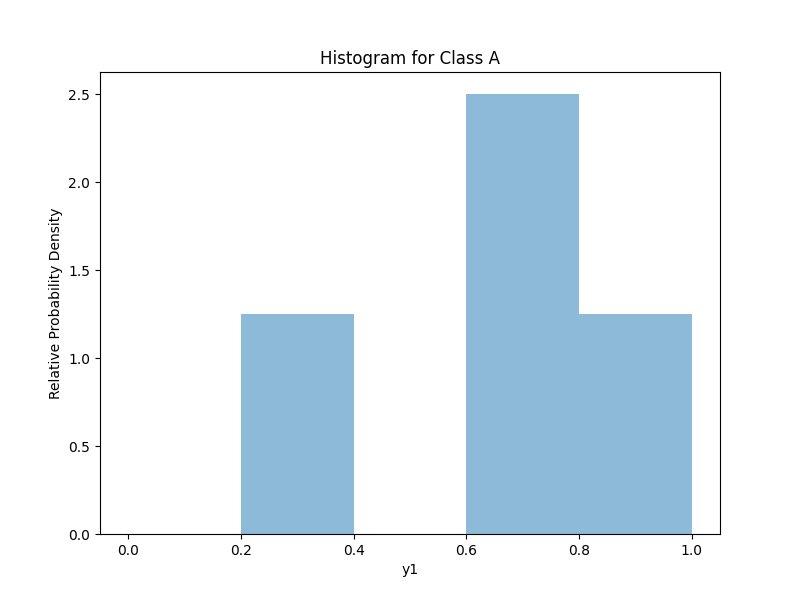
\includegraphics[width=\linewidth]{images/histogram_A.png}
    \caption{Histograma de $y_1$ para $y_{out} = A$}
    \label{fig:histogram_A}
  \end{subfigure}
  \hfill
  \begin{subfigure}{0.45\textwidth}
    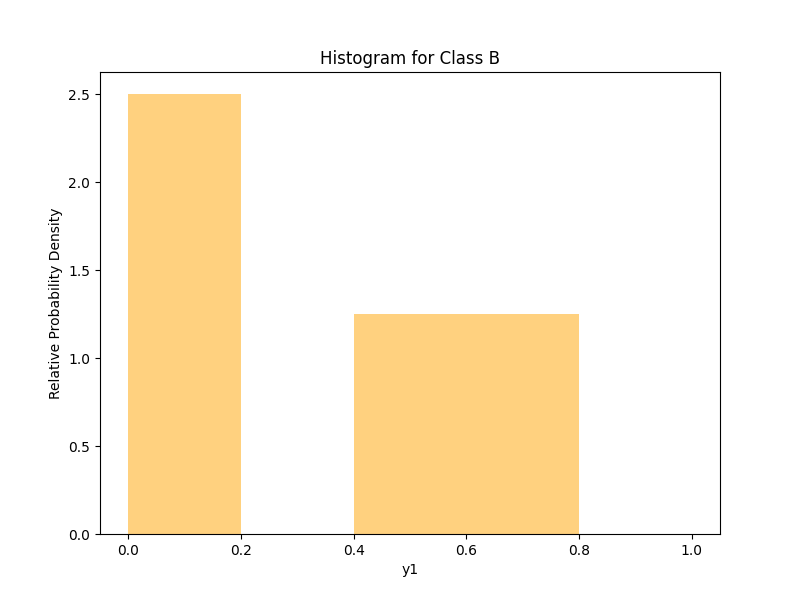
\includegraphics[width=\linewidth]{images/histogram_B.png}
    \caption{Histograma de $y_1$ para $y_{out} = B$}
    \label{fig:histogram_B}
  \end{subfigure}
  \vskip\baselineskip
  \begin{subfigure}{0.45\textwidth}
    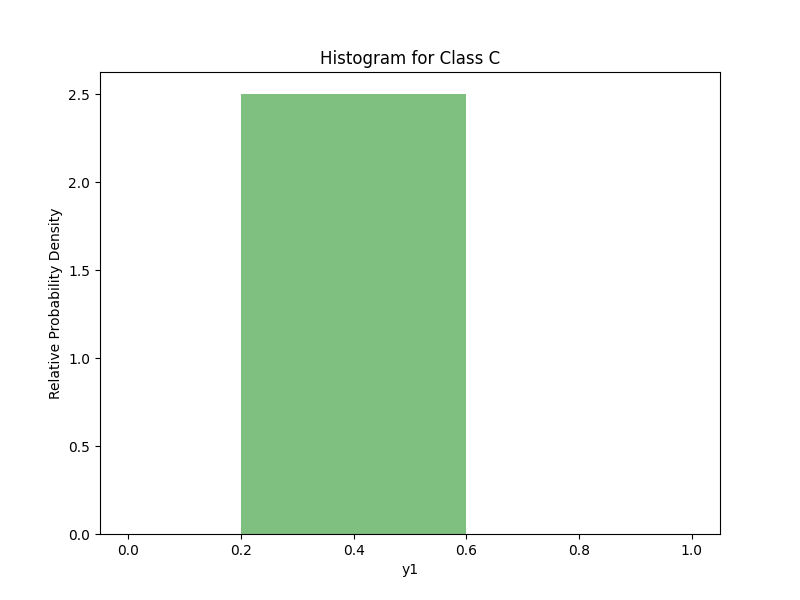
\includegraphics[width=\linewidth]{images/histogram_C.png}
    \caption{Histograma de $y_1$ para $y_{out} = C$}
    \label{fig:histogram_C}
  \end{subfigure}
  \hfill
  \begin{subfigure}{0.45\textwidth}
    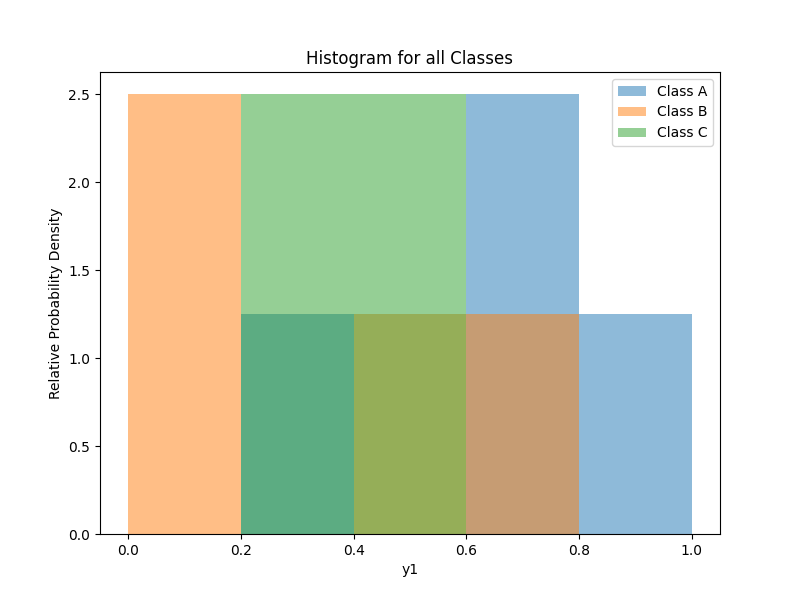
\includegraphics[width=\linewidth]{images/histogram_all.png}
    \caption{Histogramas de $y_1$ para $y_{out} = A$, $y_{out} = B$ e $y_{out} = C$}
    \label{fig:histogram_all}
  \end{subfigure}
  \caption{Histogramas de $y_1$ condicionados a $y_{out}$}
  \label{fig:histograms}
\end{figure}

Usando o critério da probabilidade máxima, podemos concluir que a classe predominante em cada bin é a classe que tem maior altura no bin, referido na tabela acima.
Deste modo e usando este critério como root split, podemos desenhar a árvore de decisão:

\begin{center}
  \begin{forest}
    for tree={
      edge={->},
      parent anchor=south,
      child anchor=north,
      align=center,
      base=top,
      draw,
      font=\sffamily,
      s sep=35mm, % Vertical separation between siblings
      l sep=10mm, % Horizontal separation between parent and child nodes
    }
    [$y_1$, circle
      [B, edge label={node[midway,above]{ $[0, 0.2[ $}}, diamond]
      [C, edge label={node[midway,above]{ $[0.2, 0.6[ $}}, diamond]
      [A, edge label={node[midway,above]{ $ [0.6, 1.0[$}}, diamond]
    ]
  \end{forest}
  
\end{center}

Anteriormente, usámos a o ganho de informação com entropia para escolher a variável que iria ser usada para o root split.
Contudo, outros métodos podem ser utilizados. Neste caso, podemos verificar que usando probabilidades condicionadas também conseguimos construir uma árvore de decisão.
No exemplo acima, apenas usámos a variável $y_1$ para construir a árvore de decisão, mas poderíamos usar mais variáveis.





\newpage

\section*{Componente de Programação}

\subsection*{Imports}

\begin{lstlisting}[language=Python]
  import sklearn as sk
  from sklearn.feature_selection import f_classif
  from sklearn.model_selection import train_test_split
  from sklearn import tree
  import numpy as np
  import pandas as pd
  import matplotlib.pyplot as plt
  import seaborn as sns
  from pathlib import Path
  from scipy.io.arff import loadarff
\end{lstlisting}

\subsection*{Dataset}

\begin{lstlisting}[language=Python]
  IMAGES_DIR = Path('images')
  DATA_DIR = Path('data')
  DATA_FILE = 'column_diagnosis.arff'
  DATA_PATH = DATA_DIR / DATA_FILE
  data = loadarff(DATA_PATH)
  df = pd.DataFrame(data[0])
  df['class'] = df['class'].str.decode('utf-8')
  # Show the first 5 rows
  df.head()
\end{lstlisting}

\subsection*{Question 1}

\subsubsection*{F-Score}

\begin{lstlisting}[language=Python]
  X = df.drop('class', axis=1)
  y = df['class']
  f_statistic, p_values = f_classif(X, y)

  f_statistic_df = pd.DataFrame({'feature': X.columns,
                                'F': f_statistic,
                                'p-value': p_values})
  f_statistic_df.sort_values('p-value')

  highest_discriminative_feature = f_statistic_df['feature'][f_statistic_df['F'].idxmax()]
  lowest_discriminative_feature = f_statistic_df['feature'][f_statistic_df['F'].idxmin()]

  print(f_statistic_df.sort_values('p-value'))
  print("\n")
  print(f"Variable with the highest F-statistic and lowest p_value: {highest_discriminative_feature}\n")
  print(f"Variable with the lowest F-statistic and highest p_value: {lowest_discriminative_feature}\n")

\end{lstlisting}

\begin{lstlisting}[language=Python]
Variable with the highest F-statistic and lowest p_value: degree_spondylolisthesis

Variable with the lowest F-statistic and highest p_value: pelvic_radius
\end{lstlisting}

\subsubsection*{Class Conditional probability density functions}
\begin{lstlisting}[language=Python]
  # Plot the class-conditional probability density functions for the two selected features
  plt.figure(figsize=(12, 6))
  
  for class_name in df['class'].unique():
      sns.kdeplot(df[df['class'] == class_name][highest_discriminative_feature], label=class_name)
  
  plt.title(f"Class Conditional Probability Density Function for {highest_discriminative_feature}")
  plt.xlabel(highest_discriminative_feature)
  plt.ylabel('Probability density')
  plt.legend()
  plt.savefig(IMAGES_DIR / 'prob_dens_highest_discriminative_feature.png')
  plt.show()
  
  plt.figure(figsize=(12, 6))
  for class_name in df['class'].unique():
      sns.kdeplot(df[df['class'] == class_name][lowest_discriminative_feature], label=class_name)
  
  plt.title(f"Class Conditional Probability Density Function for {lowest_discriminative_feature}")
  plt.xlabel(lowest_discriminative_feature)
  plt.ylabel('Probability density')
  plt.legend()
  plt.savefig(IMAGES_DIR /'prob_dens_lowest_discriminative_feature.png')
  plt.show()
\end{lstlisting}

\begin{figure}[H]
  \centering
  \begin{subfigure}{0.55\textwidth}
    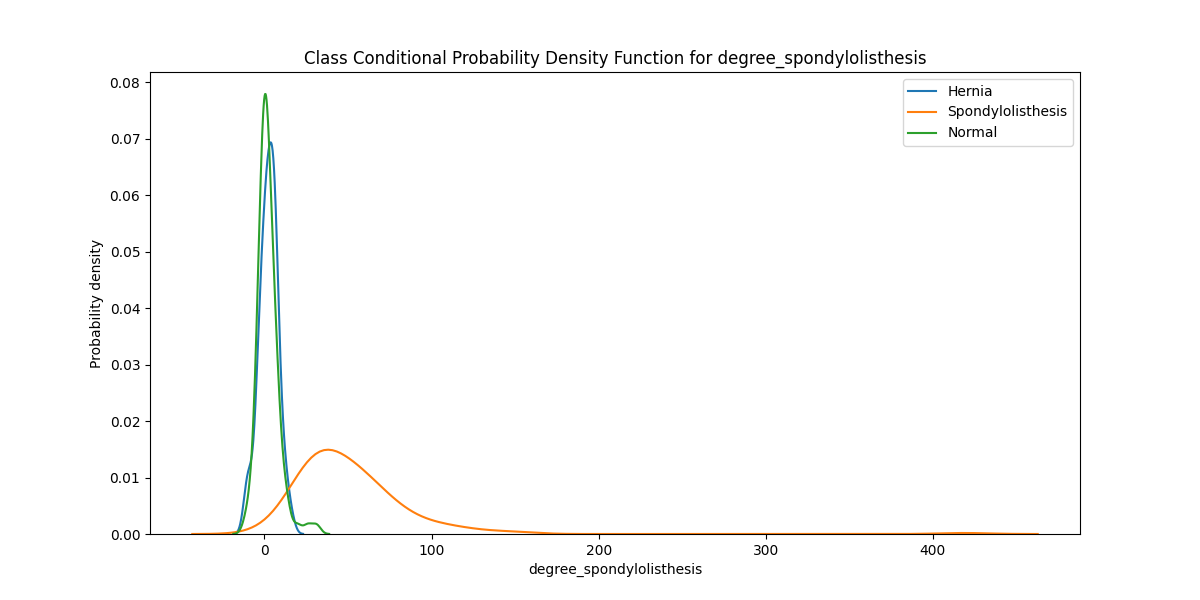
\includegraphics[width=\linewidth]{images/prob_dens_highest_discriminative_feature.png}
  \end{subfigure}
  \begin{subfigure}{0.55\textwidth}
    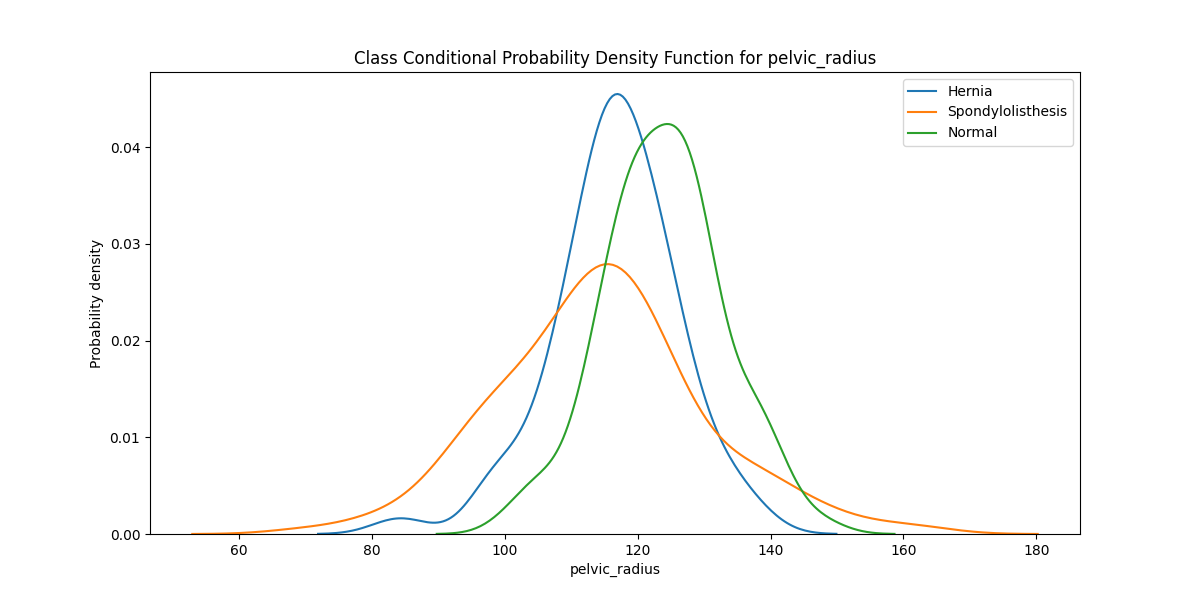
\includegraphics[width=\linewidth]{images/prob_dens_lowest_discriminative_feature.png}
  \end{subfigure}
\end{figure}

\subsubsection*{Question 2}
\begin{lstlisting}[language=Python]
  # Load and partition data
  X_train, X_test, y_train, y_test = train_test_split(X,
                                                      y,
                                                      train_size=0.7,
                                                      random_state=0,
                                                      stratify=y)
  
  # Define the range of depth limits and number of runs to average over
  depths = [1, 2, 3, 4, 5, 6, 8, 10]
  runs = 10
  
  # Arrays to keep Acc Values
  train_acc = np.zeros((runs, len(depths))) # This is going to be a 10x8 array, because we want to keep all the accuracies for each run
  test_acc = np.zeros((runs, len(depths)))
  
  # Loop over the runs
  for j, depth in enumerate(depths): # Need enumerate since we need to index the depths to keep in arrays
      for i in range(runs):
          # Learn Classifier
          predictor = tree.DecisionTreeClassifier(max_depth=depth)
          predictor.fit(X_train, y_train)
  
          # Predict on train and test set
          y_predicted_train = predictor.predict(X_train)
          y_predicted_test = predictor.predict(X_test)
  
          # Compute accuracy
          train_acc[i, j] = sk.metrics.accuracy_score(y_train, y_predicted_train)
          test_acc[i, j] = sk.metrics.accuracy_score(y_test, y_predicted_test)
  
  # Compute mean and standard deviation for train and test accuracies
  train_acc_mean = np.mean(train_acc, axis=0)
  train_acc_std = np.std(train_acc, axis=0)
  test_acc_mean = np.mean(test_acc, axis=0)
  test_acc_std = np.std(test_acc, axis=0)
  
  # Plot Optional
  plt.figure(figsize=(10, 5))
  plt.title('Accuracy vs. Depth Limit with 10 runs per depth limit')
  plt.errorbar(depths, train_acc_mean, yerr=train_acc_std, label='Train Accuracy')
  plt.errorbar(depths, test_acc_mean, yerr=test_acc_std, label='Test Accuracy')
  plt.xlabel('Depth Limit')
  plt.ylabel('Accuracy')
  plt.legend()
  plt.savefig(IMAGES_DIR /'accuracy_vs_depth_limit.png')
  plt.show()
  
  
  # Plot the Exercise without Optional Part
  plt.figure(figsize=(10, 5))
  plt.title('Accuracy vs. Depth Limit with 1 runs per depth limit')
  plt.plot(depths, train_acc[0], label='Train Accuracy') # Selecting the first run for each depth limit
  plt.plot(depths, test_acc[0], label='Test Accuracy')
  plt.xlabel('Depth Limit')
  plt.ylabel('Accuracy')
  plt.legend()
  plt.savefig(IMAGES_DIR /'accuracy_vs_depth_limit_without_optional.png')
  plt.show()
  
\end{lstlisting}


\begin{figure}[H]
  \centering
  \begin{subfigure}{0.55\textwidth}
    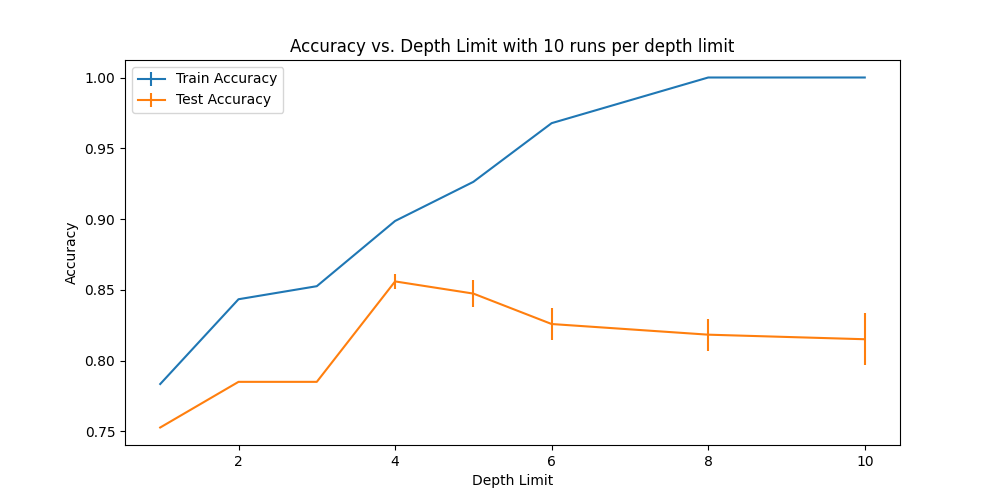
\includegraphics[width=\linewidth]{images/accuracy_vs_depth_limit.png}
  \end{subfigure}
  \begin{subfigure}{0.55\textwidth}
    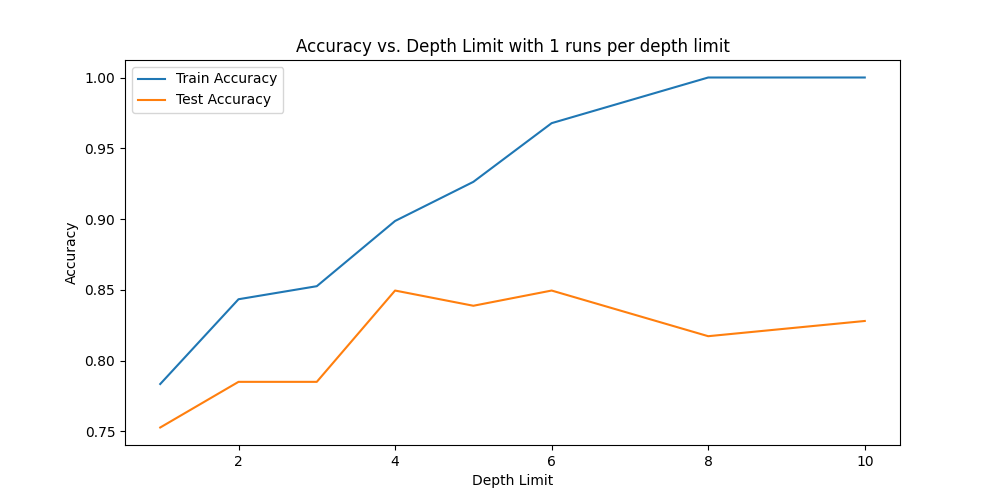
\includegraphics[width=\linewidth]{images/accuracy_vs_depth_limit_without_optional.png}
  \end{subfigure}
\end{figure}

\subsubsection*{Question 3}
Como se vê em ambos os gráficos, a precisão de treino aumenta à medida que o limite de profundidade da árvore de decisão aumenta. No entanto, a precisão de teste aumenta até um certo limite de profundidade (neste caso, cerca de 4 ou 5) e depois começa a diminuir. Isto acontece porque a árvore de decisão está a dar overfit aos dados de treino e não está a aprender de modo a corretamente avaliar os dados de teste.
No que toca à parte opcional, também podemos ver que o desvio padrão geralmente é pequeno no caso do treino, o que indica que os resultados são consistentes em diferentes inicializações aleatórias dos dados. No entanto, o desvio padrão é maior para os dados de teste, o que indica que os dados de teste são mais sensíveis à inicialização aleatória dos dados.

\subsubsection*{Question 4}

    \begin{lstlisting}[language=Python]
      # Learn a decision tree with a minimum number of samples per leaf = 20
      predictor = tree.DecisionTreeClassifier(min_samples_leaf=20,
                                              random_state=0)
      
      # Fit all the data
      predictor.fit(X, y)
      
      # Plot the tree
      plt.figure(figsize=(20, 10))
      tree.plot_tree(predictor,
                      feature_names=X.columns,
                      filled=True,
                      class_names=predictor.classes_)
      plt.title('Decision Tree with Minimum Samples per Leaf = 20', fontsize=20)
      plt.savefig(IMAGES_DIR / 'decision_tree_min_samples_leaf_20.png')
      plt.show()
    \end{lstlisting}

    \begin{figure}[H]
      \centering
      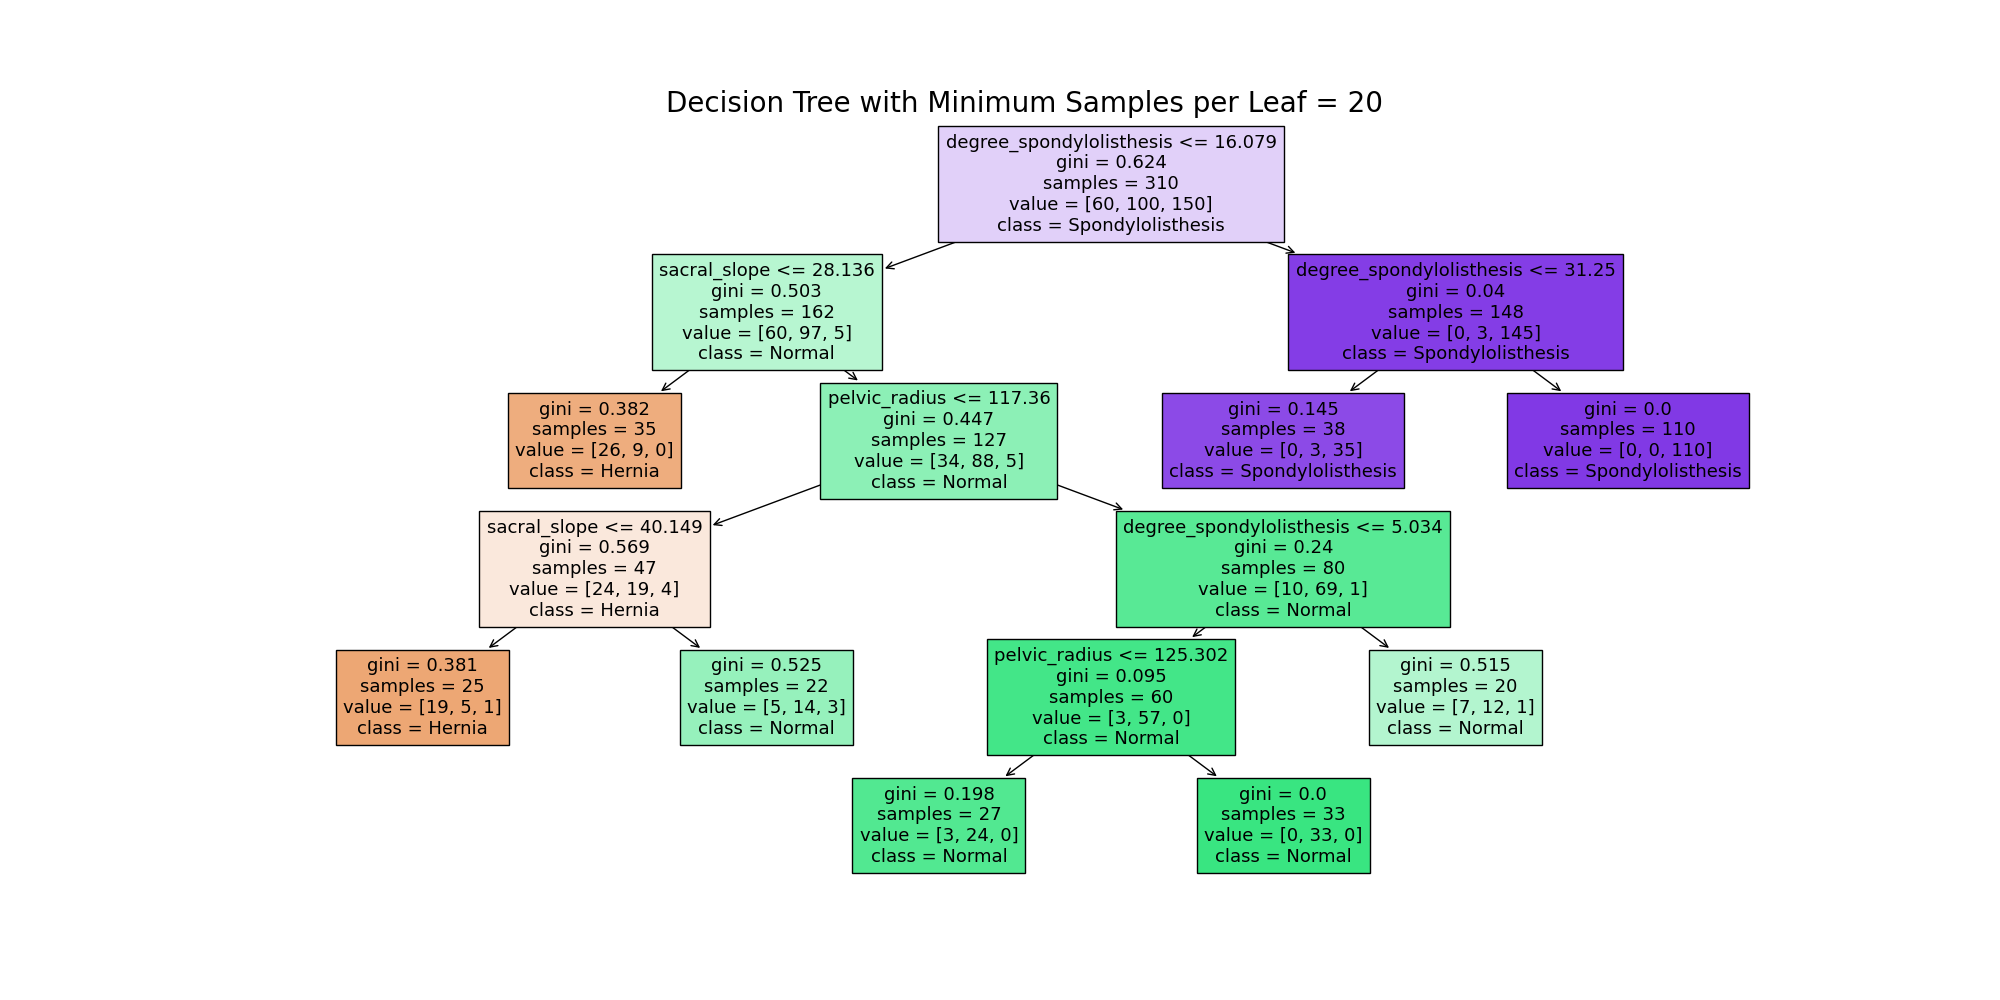
\includegraphics[width=1\linewidth]{images/decision_tree_min_samples_leaf_20.png}
    \end{figure}

De acordo com a árvore de decisão construída na alínea anterior, existem dois casos nos quais o indivíduo em questão tem um outcome de diagnóstico com Hérnia. Em primeiro lugar temos degree spondylolisthesis $\leq 16.079$ e sacral slope $\leq 28.136$. 
Em segundo lugar, temos degree spondy|olisthesis $\leq 16.079$, sacral slope $> 28.136$, pelvic radius $ \leq 117.36$ e sacral slope $\leq 40.149$.





\end{document}